%!TEX program = xelatex
\documentclass[dvipsnames, svgnames,a4paper,11pt]{article}
% ----------------------------------------------------
%   中山大学物理与天文学院本科实验报告模板
%   作者:Huanyu Shi,2019级
%   知乎:https://www.zhihu.com/people/za-ran-zhu-fu-liu-xing
%   Github:https://github.com/Huanyu-Shi/SYSU-SPA-Labreport-Template
%   Last update : 2023.4.10
% ----------------------------------------------------

% ----------------------------------------------------- 
%	加边框的命令
%	参考:https://tex.stackexchange.com/questions/531559/how-to-add-the-page-border-for-first-two-pages-in-latex
\usepackage{tikz}
\usetikzlibrary{calc}
\usepackage{eso-pic}
\AddToShipoutPictureBG{%
\begin{tikzpicture}[overlay,remember picture]
\draw[line width=0.6pt] % 边框粗细
    ($ (current page.north west) + (0.6cm,-0.6cm) $)
    rectangle
    ($ (current page.south east) + (-0.6cm,0.6cm) $); % 边框位置
\end{tikzpicture}}


\usepackage{xcolor}
\definecolor{c1}{HTML}{2752C9} % 目录颜色
\definecolor{c2}{RGB}{190,20,83} % 引用颜色

\usepackage{ctex}
\usepackage[top=28mm,bottom=28mm,left=15mm,right=15mm]{geometry}
\usepackage{hyperref} 
\hypersetup{
	colorlinks,
	linktoc = section, % 超链接位置,选项有section, page, all
	linkcolor = c1, % linkcolor 目录颜色
	citecolor = c1  % citecolor 引用颜色
}
\usepackage{amsmath,enumerate,multirow,float}
\usepackage{tabularx}
\usepackage{tabu}
\usepackage{subfig}
\usepackage{fancyhdr}
\usepackage{graphicx}
\usepackage{wrapfig}  
\usepackage{physics}
\usepackage{appendix}
\usepackage{amsfonts}

%
\usepackage{tcolorbox}
\tcbuselibrary{skins,breakable}
\newtcolorbox{tbox}[2][]{
    colframe=black!70!,
    breakable,
    enhanced,
	boxrule =0.5pt,
    title = {#2},
    fonttitle = \large\kaishu\bfseries,
	drop fuzzy shadow,
    #1
}
\newtcolorbox[auto counter,number within=section]{question}[1][]{
  top=2pt,bottom=2pt,arc=1mm,
  boxrule=0.5pt,
%   frame hidden,
  breakable,
  enhanced, %跨页后不会显示下边框
  coltitle=c1!80!gray,
  colframe=c1,
  colback=c1!3!white,
  drop fuzzy shadow,
  title={思考题~\thetcbcounter:\quad},
  fonttitle=\bfseries,
  attach title to upper,
  #1
}
\newcommand{\setLhead}[1]{%
  \lhead{{\color{gray}\kaishu #1}} % 定义新的命令,设置右边页眉的内容
}
\newcommand{\setRhead}[1]{%
  \rhead{{\color{gray}\kaishu #1}} % 定义新的命令,设置右边页眉的内容
}
% ---------------------------------------------------------------------
%	利用cleveref改变引用格式,\cref是引用命令
\usepackage{cleveref}
\crefformat{figure}{#2{\textcolor{c2}{图 #1}}#3} % 图片的引用格式
\crefformat{equation}{#2{(\textcolor{c2}{#1})}#3} % 公式的引用格式
\crefformat{table}{#2{\textcolor{c2}{表 #1}}#3} % 表格的引用格式


% ---------------------------------------------------------------------
%	页眉页脚设置
\fancypagestyle{plain}{\pagestyle{fancy}}
\pagestyle{fancy}
\setLhead{中山大学物理与天文学院基础物理实验预习报告}
%\lhead{\kaishu 中山大学物理与天文学院物理实验\uppercase\expandafter{\romannumeral3}} % 左边页眉,学院 + 课程
%\rhead{{\color{gray}\kaishu Template 实验报告模板}} % 右边页眉,实验报告标题
\setRhead{实验1\hspace{1pt}冰的熔化热测量}
\cfoot{\thepage} % 页脚,中间添加页码


% ---------------------------------------------------------------------
%	对目录、章节标题的设置
\renewcommand{\contentsname}{\centerline{\huge 目录}}
\usepackage{titlesec}
\usepackage{titletoc}
% \titleformat{章节}[形状]{格式}{标题序号}{序号与标题间距}{标题前命令}[标题后命令]
\titleformat{\section}{\centering\LARGE\songti}{}{1em}{}

% ---------------------------------------------------------------------
%   listing代码环境设置
\usepackage{listings}
\lstloadlanguages{python}
\lstdefinestyle{pythonstyle}{
backgroundcolor=\color{gray!5},
language=python,
frameround=tftt,
frame=shadowbox, 
keepspaces=true,
breaklines,
columns=spaceflexible,                   
basicstyle=\ttfamily\small, % 基本文本设置,字体为teletype,大小为scriptsize
keywordstyle=[1]\color{c1}\bfseries, 
keywordstyle=[2]\color{Red!70!black},   
stringstyle=\color{Purple},       
showstringspaces=false,
commentstyle=\ttfamily\scriptsize\color{green!40!black},%注释文本设置,字体为sf,大小为smaller
tabsize=2,
morekeywords={as},
morekeywords=[2]{np, plt, sp},
numbers=left, % 代码行数
numberstyle=\it\tiny\color{gray}, % 代码行数的数字字体设置
stepnumber=1,
rulesepcolor=\color{gray!30!white}
}




% ---------------------------------------------------------------------
%	其他设置
\def\degree{${}^{\circ}$} % 角度
\graphicspath{{./images/}} % 插入图片的相对路径
\allowdisplaybreaks[4]  %允许公式跨页 % 导入模板的相关设置
\usepackage{lipsum}
\usepackage{indentfirst}
\usepackage{pdfpages}
\usepackage{multirow}
\usepackage{subfig}
\usepackage{graphicx}
\usepackage{float} 
\usepackage{circuitikz}
\definecolor{mygreen}{rgb}{0,0.6,0}
\definecolor{mygray}{rgb}{0.5,0.5,0.5}
\definecolor{mymauve}{rgb}{0.58,0,0.82}
\lstset{
 backgroundcolor=\color{lightgray}, 
 basicstyle = \footnotesize,       
 breakatwhitespace = false,        
 breaklines = true,                 
 captionpos = b,                    
 commentstyle = \color{mygreen}\bfseries,
 extendedchars = false,             
 frame =shadowbox, 
 framerule=0.5pt,
 keepspaces=true,
 keywordstyle=\color{blue}\bfseries, % keyword style
 language = C++,                     % the language of code
 otherkeywords={string}, 
 numbers=left, 
 numbersep=5pt,
 numberstyle=\tiny\color{mygray},
 rulecolor=\color{black},         
 showspaces=false,  
 showstringspaces=false, 
 showtabs=false,    
 stepnumber=1,         
 stringstyle=\color{mymauve},        % string literal style
 tabsize=2,          
 title=\lstname                      
}
\renewcommand{\d}{\mathrm{d}}


%---------------------------------------------------------------------
%	正文
%---------------------------------------------------------------------
\setRhead{AA4 传感器综合实验}%实验名称
\begin{document}


\begin{table}
	\renewcommand\arraystretch{1.7}
	\begin{tabularx}{\textwidth}{
		|X|X|X|X
		|X|X|X|X|}
	\hline
	\multicolumn{2}{|c|}{预习报告}&\multicolumn{2}{|c|}{实验记录}&\multicolumn{2}{|c|}{分析讨论}&\multicolumn{2}{|c|}{总成绩}\\
	\hline
	 25& &30  & &25  & &80& \\
	\hline
	\end{tabularx}
\end{table}


\begin{table}
	\renewcommand\arraystretch{1.7}
	\begin{tabularx}{\textwidth}{|X|X|X|X|}
	\hline
	专业:& 物理学类 &年级:& 2023级\\
	\hline
	姓名:& 姚昊廷  & 学号:&22322091\\
	\hline
	日期:& 2024.10.24& 教师签名:& \\
	\hline
	\end{tabularx}
\end{table}

\begin{center}
	\LARGE AA4 传感器综合实验
\end{center}

\textbf{【实验报告注意事项】}
\begin{enumerate}
	\item 实验报告由三部分组成:
	\begin{enumerate}
		\item 预习报告:(提前一周)认真研读\underline{\textbf{实验讲义}},弄清实验原理;实验所需的仪器设备、用具及其使用(强烈建议到实验室预习),完成课前预习思考题;了解实验需要测量的物理量,并根据要求提前准备实验记录表格(第一循环实验已由教师提供模板,可以打印)。预习成绩低于10分(共20分)者不能做实验。
	    \item 实验记录:认真、客观记录实验条件、实验过程中的现象以及数据。实验记录请用珠笔或者钢笔书写并签名(\textcolor{red}{\textbf{用铅笔记录的被认为无效}})。\textcolor{red}{\textbf{保持原始记录,包括写错删除部分,如因误记需要修改记录,必须按规范修改。}}(不得输入电脑打印,但可扫描手记后打印扫描件);离开前请实验教师检查记录并签名。
	    \item 分析讨论:处理实验原始数据(学习仪器使用类型的实验除外),对数据的可靠性和合理性进行分析;按规范呈现数据和结果(图、表),包括数据、图表按顺序编号及其引用;分析物理现象(含回答实验思考题,写出问题思考过程,必要时按规范引用数据);最后得出结论。
	\end{enumerate}
	\textbf{实验报告就是将预习报告、实验记录、和数据处理与分析合起来,加上本页封面。}
	\item 每次完成实验后的一周内交\textbf{实验报告}(特殊情况不能超过两周)。
	\item 除实验记录外,实验报告其他部分建议双面打印。
\end{enumerate}

{\textbf{【实验安全与实验室注意事项】}
\begin{enumerate}
	\item 所有实验均在 ELVIS 板上接线,调节、测量读数由电脑控制完成。
	\item {\color{red}做一个小实验,都请先连好线路、并确保检查无误(电源正负极没有接反;电线都插紧;没有短路),
    再打开 ELVIS 板右上方 PROTO 电源,以防烧坏仪器。}
	\item 每做完一个实验,请关掉右上 PROTO 电源、拆掉导线、将电路开关断路,再开始下一个实验连线。
    \item 电压/电阻/电流表请选择与待测信号最接近的量程,否则会有较大误差(仪器制造问题)。
    \item ELVIS 板四孔脚标 12 内部连通,脚标 34 内部连通,脚标 12 与脚标 34 之间不连通。
    
\end{enumerate}}

\clearpage
\tableofcontents
\clearpage

\setcounter{section}{0}
\section{AA4 传感器综合实验 \textbf{预习报告}}
	
\subsection{实验目的}
\begin{enumerate}
	\item 了解包括光敏电阻等数种传感器元件的原理、特性。
	\item 学习使用 ELVIS 并了解其测量原理。
	\item 练习规范连接电路、测量电压与电流。
	\item 练习规范记录实验结果和数据处理。
\end{enumerate}

\subsection{仪器用具}
\begin{table}[htbp]
	\centering
	\renewcommand\arraystretch{1.6}
	% \setlength{\tabcolsep}{10mm}
	\begin{tabular}{p{0.05\textwidth}|p{0.20\textwidth}|p{0.05\textwidth}|p{0.5\textwidth}}
	\hline
	编号& 仪器用具名称 & 数量 &  主要参数(型号,测量范围,测量精度等) \\
	\hline
	1&ELVI传感器实验电路板&1台 &\\
	\hline
	2&传感器实验套件&1套&光敏电阻,PIN二极管\\
	\hline
	3&鳄鱼夹表笔套& 2 & \\
	\hline
	4&面包板测试线&20 &  \\
	\hline
\end{tabular}
\end{table}

\textbf{【实验内容】}\\

光敏电阻特性实验:定量记录结果\\
PIN 二极管特性实验:定量记录结果。\\
霍尔 IC 电机转速实验:定量记录结果

\textbf{【原理概述】}
\begin{question}
    什么是暗电阻、亮电阻?什么是暗电流、亮电流、光电流?什么是偏置电压?
    \tcblower
    暗电阻:光敏电阻在不受光照时的阻值。\\
    亮电阻:光敏电阻在受光照时的阻值。\\
    暗电流:光敏电阻不受光照射时的流过的电流。\\
    亮电流:光敏电阻在受光照射时的流过的电流。\\
    光电流=亮电流-暗电流\\
    偏置电压是电源提供的直流电压大小。
\end{question}

\begin{question}
    画出测量光敏电阻的简单电路图。
    \tcblower
    \begin{figure}[H]     
		\centering  %图片全局居中     
		\subfloat[光敏电阻暗电流测量电路图]{     
			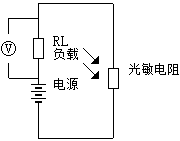
\includegraphics[width=0.5\textwidth]{光敏暗电流.png}}   
			
		\subfloat[光敏电阻亮电流测量电路图]{         
			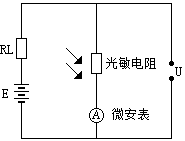
\includegraphics[width=0.5\textwidth]{光敏光电流.png}}     
	\end{figure}  
\end{question}

\begin{question}
    画出测量PIN二极管的简单电路图。
    \tcblower
    \begin{figure}[H]     
		\centering  %图片全局居中     
		\subfloat[PIN光电二极管暗电流测试原理图]{     
			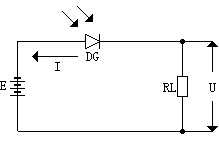
\includegraphics[width=0.5\textwidth]{PIN暗电流.png}}   
			
            \subfloat[PIN光电二极管亮电流测试原理图]{     
                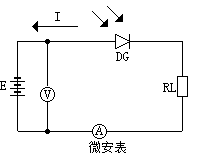
\includegraphics[width=0.5\textwidth]{PIN亮电流.png}}     
	\end{figure}  
\end{question}

\begin{question}
   什么是霍尔效应?什么是单级霍尔效应开关?
    \tcblower
    \textbf{霍尔效应:}  霍尔效应是指在电流通过导体或半导体时,垂直于电流方向施加磁场,导致材料内出现横向电压的现象。具体来说,当带电粒子(如电子或正孔)在磁场中运动时,磁场对它们施加的洛伦兹力会使它们偏离直线运动轨迹,造成电荷在材料的某一侧积聚,从而在材料的横向产生电压差。
    这种现象被称为霍尔电压(Hall Voltage),并且其方向与电流和磁场的方向遵循右手法则。
    霍尔效应广泛应用于测量磁场、传感器、磁场开关等领域。

    \textbf{单级霍尔效应开关:}单级霍尔效应开关是一种基于霍尔效应原理工作的开关装置。它的主要特点是能够在检测到磁场时,开关状态发生变化(例如,开启或关闭电路)。通常情况下,它由霍尔传感器、放大器和输出驱动电路组成。
    在磁场强度大于$B_{OP}$时晶体管开启,小于$B_{OP}$时晶体管关闭。
\end{question}



\clearpage
\setLhead{中山大学物理与天文学院基础物理实验记录}
\begin{table}
	\renewcommand\arraystretch{1.7}
	\centering
	\begin{tabularx}{\textwidth}{|X|X|X|X|}
	\hline
	专业:& 物理学类 &年级:& 2023级 \\
	\hline
	姓名:& 姚昊廷 &学号:&22322091  \\
	\hline
	室温:&25.0$^\circ$C&实验地点:&A507\ D2\\
	\hline
	学生签名:& & 评分: &\\
	\hline
	实验时间:& 2024.10.24& 教师签名:&\\
	\hline
	\end{tabularx}
\end{table}

\section{AA4 传感器综合实验 \textbf{实验记录}}
\textbf{【光敏电阻实验步骤与记录】}
由于仪器灵敏度较差、耗费时间较长,不再测量光敏器件的暗电流。仅观察其光照特性。\\
\textbf{一.观测光敏电阻的伏安特性}

按照讲义连好电路。将面板上的“电流表”插孔连线到左侧电流测量表。检查无误后,再打开ELVIS PROTO 电源。

采用白光照射光敏电阻(应使得光源尽可能靠近电阻,白光直射电阻;如引脚过长,请折弯引脚)。调节偏置电源电压(VPS供电)为 4V、6V、8V、10V、12V(在其附近即可),测量电路中电流的大小,记录如下:
\begin{table}[htbp]
	\renewcommand\arraystretch{1.7}
	\centering
    \caption{$R=20k\Omega$}
	\begin{tabularx}{\textwidth}{|X|X|X|X|X|X|}
	\hline
	偏置电源电压(V)&4 &6& 8&10&12\\
	\hline
	通过传感器的电流($\mu$A)& 164.4 &247&329&413&496  \\
	\hline
	\end{tabularx}
\end{table}

\textbf{二.测定光敏电阻的光照特性}\\
请将面板上的“电压表”插孔连线到左侧电压测量表。
请选用一种固定颜色的光源(红、绿、蓝、橙均可),偏置电压固定为 8 V,将占空比从 1\%-99\% 均匀调节(记录频率设定),RL=1k(或选用合适的RL),记录测量电压随光照改变的变化。
\begin{table}[H]
	\renewcommand\arraystretch{1.7}
	\centering
    \caption{$R=1k\Omega$,使用橙色灯}
	\begin{tabularx}{\textwidth}{|X|X|X|X|X|X|X|X|X|X|X|}
	\hline
	占空比k&1\% &12\%& 23\%&34\%&45\%&55\%&66\%&77\%&88\%&99\%\\
	\hline
	电压(V)&0.378&0.899&1.186&1.398&1.583&1.684&1.891&1.961&2.109&2.153  \\
	\hline
	\end{tabularx}
\end{table}

\textbf{二.测定光敏电阻的光谱特性}\\
请调节占空比 100\%,偏置电压固定为 8V。使用至少三种不同颜色的 LED 光源照射光敏电阻/光敏二极管,测量电压。
\begin{table}[H]
	\renewcommand\arraystretch{1.7}
	\centering
	\begin{tabularx}{\textwidth}{|X|X|X|X|}
	\hline
	光源颜色&橙&红&绿\\
	\hline
	电压(V)&2.124&2.588&1.911  \\
	\hline
	\end{tabularx}
\end{table}

\textbf{【PIN二极管特性实验步骤与记录】}\\
\textbf{一.观测 PIN 光电二极管的光照特性}\\
参照讲义中的测量电路,选择合适的测量方法(电压/电流),设计合适的 $R_L$并记录,选择E=12V。调整不同的光照占空比,测得的光生电流并填入下表中。
\begin{table}[H]
	\renewcommand\arraystretch{1.7}
	\centering
	\caption{$R_L=10M\Omega$}
	\begin{tabularx}{\textwidth}{|X|X|X|X|X|X|X|}
	\hline
	光照占空比&0 &20\%& 40\%&60\%&80\%&100\%\\
	\hline
	光生电流($\mu$A)&0.002&0.290&0.793&1.159&1.215&1.231  \\
	\hline
	\end{tabularx}
\end{table}

\textbf{二.观测 PIN 光电二极管的伏安特性}\\
根据上题钟的测量电路,RL 选择合适值并记录,占空比50\%,保持光照度不变,分别测量计算不同 E 值时的光生电流,填入下表。然后调整占空比为 100\%,保持光照度不变,分别测量不同 E 值时的光生电流,填入下表。
\begin{table}[H]
	\renewcommand\arraystretch{1.7}
	\centering
	\caption{$R_L=1k\Omega$}
	\begin{tabularx}{\textwidth}{|X|X|X|X|X|X|X|X|}
	\hline
	偏压&0 &-2&-4&-6&-8&-10&-12\\
	\hline
	光生电流($\mu$A)(50\%)&0.059&0.240&0.419&0.609&0.797&0. 982&1.163\\
	\hline
	光生电流($\mu$A)(100\%)&0.062&0.229&0.430&0.629&0.829&1.029&1.228\\
	\hline
	\end{tabularx}
\end{table}

\textbf{【霍尔 IC 测速实验步骤与记录】}\\
\textbf{一.观测开环系统直流电机转速与控制电压的关系}\\
\begin{table}[H]
	\renewcommand\arraystretch{1.7}
	\centering
	\begin{tabularx}{\textwidth}{|X|X|X|X|X|X|X|}
	\hline
	驱动电压(V)&1.5 &1.6&1.7&1.8&1.9&2.0\\
	\hline
	电机转速(rpm)&750.046&862.281&943.429&1100.15&1249.81&1389.96\\
	\hline
	\end{tabularx}
\end{table}
\textbf{一.观测闭环系统 PID 控制参数与转速调节的关系(选做)}\\
据讲义中电路图连接电路,设定合适的目标转速为{\color{red}2100rpm},分别合理配置比例+积分+微分(PID)控制器,观测不同PID参数下的阶跃运动控制曲线。

\subsection{实验过程中遇到的问题记录}



\clearpage
\setLhead{中山大学物理与天文学院基础物理实验分析与讨论}
\begin{table}
	\renewcommand\arraystretch{1.7}
	\begin{tabularx}{\textwidth}{|X|X|X|X|}
	\hline
	专业:& 物理学 &年级:& 2023级\\
	\hline
	姓名: &姚昊廷 & 学号:& 22322091\\
	\hline
    日期:&2024.10.24 & 评分: &\\
	\hline
	\end{tabularx}
\end{table}

\section{AA4 传感器综合实验 分析与讨论}
\textbf{一、观测光敏电阻的伏安特性}\\
通过五次测量,得到传感器电阻平均结果为$\text{R}=(4269.03\pm 55.46)\Omega$\\
{\color{red}*参照《误差理论与数据处理》对五次测量的结果进行误差分析,利用罗曼诺夫斯基准则,取显著度α=0.01,对数据列进行粗大误差判断(给出过程),剔除粗大误差后,给出最终算数平均值和平均值标准差。列举不少于三项测量过程中的系统误差来源。}\\
五次测量得到的R分别为4330.90$\Omega$,4291.50$\Omega$,4316.11$\Omega$,4213.08$\Omega$,4193.55$\Omega$。\\
去掉x0后的新标准差为59.4198均值为4253.56\\
去掉x1后的新标准差为70.1104均值为4263.41\\
去掉x2后的新标准差为64.8244均值为4257.26\\
去掉x3后的新标准差为61.8182均值为4283.01\\
去掉x4后的新标准差为52.4611均值为4287.9\\
查t分布表知$n=4,\alpha=0.01$时$K=4.604$
由此可知,测得的阻值均不为粗大误差,判断的cpp代码见附录。
最终算数平均值为4269.03$\Omega$平均值标准差为55.46$\Omega$。
系统误差来源有
\begin{enumerate}
	\item 电流表内阻;
	\item 电源内阻;
	\item 数字万用表的显示精度不高。
\end{enumerate}

\textbf{二、测定光敏电阻的光照特性}\\
按照电路图,光敏电阻电阻 R 与电压表读数 U 的关系为(列出公式)
$$R=R_L(\frac{E_0}{U}-1)$$
其中$E_0$为电源电动势。

由此计算$R$随占空比变化的曲线(作图)
\begin{figure}[H]
	\includegraphics*[width=\textwidth]{R占空比.png}
\end{figure}
\textbf{三. 测定光敏电阻的光谱特性}\\
\begin{table}[H]
	\renewcommand\arraystretch{1.7}
	\centering
	\begin{tabularx}{\textwidth}{|X|X|X|X|}
	\hline
	光源颜色&橙&红&绿\\
	\hline
	光源波长(大概值)/nm&600&630&550\\
	\hline
	电阻/$\Omega$&2766&2091&3186  \\
	\hline
	\end{tabularx}
\end{table}
由此得到电阻随光源波长变化图为
\begin{figure}[H]
	\includegraphics*[width=\textwidth]{电阻随波长.png}
\end{figure}

\textbf{四.作图并分析 PIN 光电二极管的光照特性曲线。}\\
\begin{figure}[H]
	\includegraphics*[width=\textwidth]{光生电流占空比.png}
\end{figure}
固定$R_L$与$E$后,PIN光电二极管的光电流随占空比增加先上升后几乎不变,上升初期显示出接近正比关系,上升末期趋近于饱和。

\textbf{五.根据测得的实验数据,作出三组PID 控制器下的阶跃响应曲线, 并进行分析比较。(选做)}\\
\begin{figure}[H]     
	\includegraphics[width=\textwidth]{0.001 0.01 0.01.png}
	\caption{$P=0.001,I=0.01,D=0.01$}  	    
\end{figure}  
\begin{figure}[H]
	\includegraphics[width=\textwidth]{0.00045 0.005 0.005.png}
	\caption{$P=0.00045,I=0.005,D=0.005$}
\end{figure}
\begin{figure}[H]
	\includegraphics[width=\textwidth]{0.00045 0.01 0.01.png}
	\caption{$P=0.00045,I=0.01,D=0.01$}
\end{figure}
$P=0.00045,I=0.01,D=0.01$时收敛最快,$P=0.001,I=0.01,D=0.01$初始振荡后来振幅越来越小趋近于目标转速,$P=0.00045,I=0.005,D=0.005$则经过两次大的振荡后迅速收敛。


\textbf{【实验后思考题】}
\begin{question}
	试举光敏电阻在日常生活中的应用事例。
	\tcblower
	\begin{enumerate}
		\item 自动灯光控制:在街道照明、庭院灯或走廊灯中,光敏电阻可以检测环境光线的强度。当光线变暗时,光敏电阻的电阻值会下降,触发电路打开灯光;而当光线变亮时,灯光自动关闭。
		\item 光控电子玩具:一些电子玩具使用光敏电阻作为光传感器,使玩具在特定光照条件下启动或关闭。例如,某些玩具车在光照下移动,而在阴暗处停止。
		\item 相机曝光控制:在一些相机中,光敏电阻被用于自动曝光控制,根据光照条件自动调整快门速度和光圈,以确保拍摄的图像具有适当的亮度。
		\item 光感应报警系统:光敏电阻可以集成到安全系统中,以检测入侵者的活动。如果某个区域的光线发生变化(例如有人通过),系统可以触发报警。
		\item 智能家居系统:在智能家居中,光敏电阻可以与其他传感器结合,自动调节窗帘或百叶窗的开合,依据外部光照强度来调节室内光线。
	\end{enumerate}
\end{question}
\begin{question}
	调研回答,光敏电阻的阻值随光照迅速减小的物理机制?
	\tcblower
	入射光(波长有上限)使材料中电子跃迁到导带(自由电子,但还未逸出材料表面成为光电子),在材料中形成电子——空穴对(载流子),大大提高导电性。即内光电效应。
\end{question}
\clearpage
% ---------------------------------------------------------------------
%   参考文献
%   注:使用参考文献时应按照xelatex->bibtex->xelatex->xelatex顺序进行编译
\phantomsection
%\addcontentsline{toc}{section}{参考文献}
\bibliographystyle{unsrt}
\bibliography{myref}
%\begin{thebibliography}{9}
	%\bibitem{ref1} 凤飞龙,黄育红,金蔚,王公正,崔致远,“外推法计算冰的熔解热的理论依据及Matlab实现方案”,《大学物理》,第42卷,第2期
%\end{thebibliography}


\clearpage
\appendix
\appendixpage
\addappheadtotoc
\subsection*{判断是否粗大误差代码}
\begin{lstlisting}[caption={}]
#include <iostream>
#include <cmath>
using namespace std;

int main() { 
    double R[5] = {4330.90024, 4291.49798, 4316.10942, 4213.07506, 4193.54839};
    
    for (int i = 0; i < 5; i++) { // 循环范围修正为 5
        double he = 0;
        double he2 = 0;
        int count = 0; // 计数器,用于计算新均值
        for (int j = 0; j < 5; j++) {
            if (i == j) { // 修正条件判断为 ==
                continue; // 跳过当前索引 i
            }
            he += R[j]; // 累加未去掉的值
            count++; // 计数未去掉的值数量
        }
        
        double junzhi = he / count; // 计算新均值
        for (int j = 0; j < 5; j++) {
            if (i == j) {
                continue; // 跳过当前索引 i
            }
            he2 += (R[j] - junzhi) * (R[j] - junzhi); // 计算方差
        }
        
        double sigma = sqrt(he2 / (count - 1)); // 使用 count-1 计算样本标准差
        if ((R[i]-junzhi)*(R[i]-junzhi)>4.604*sigma*4.604*sigma)
        {
            cout<<i<<"是粗大误差"<<endl;
        }
        
        cout << "去掉x" << i << "后的新标准差为" << sigma <<"均值为"<<junzhi<< endl;
    }
    
    return 0;
}

\end{lstlisting}
%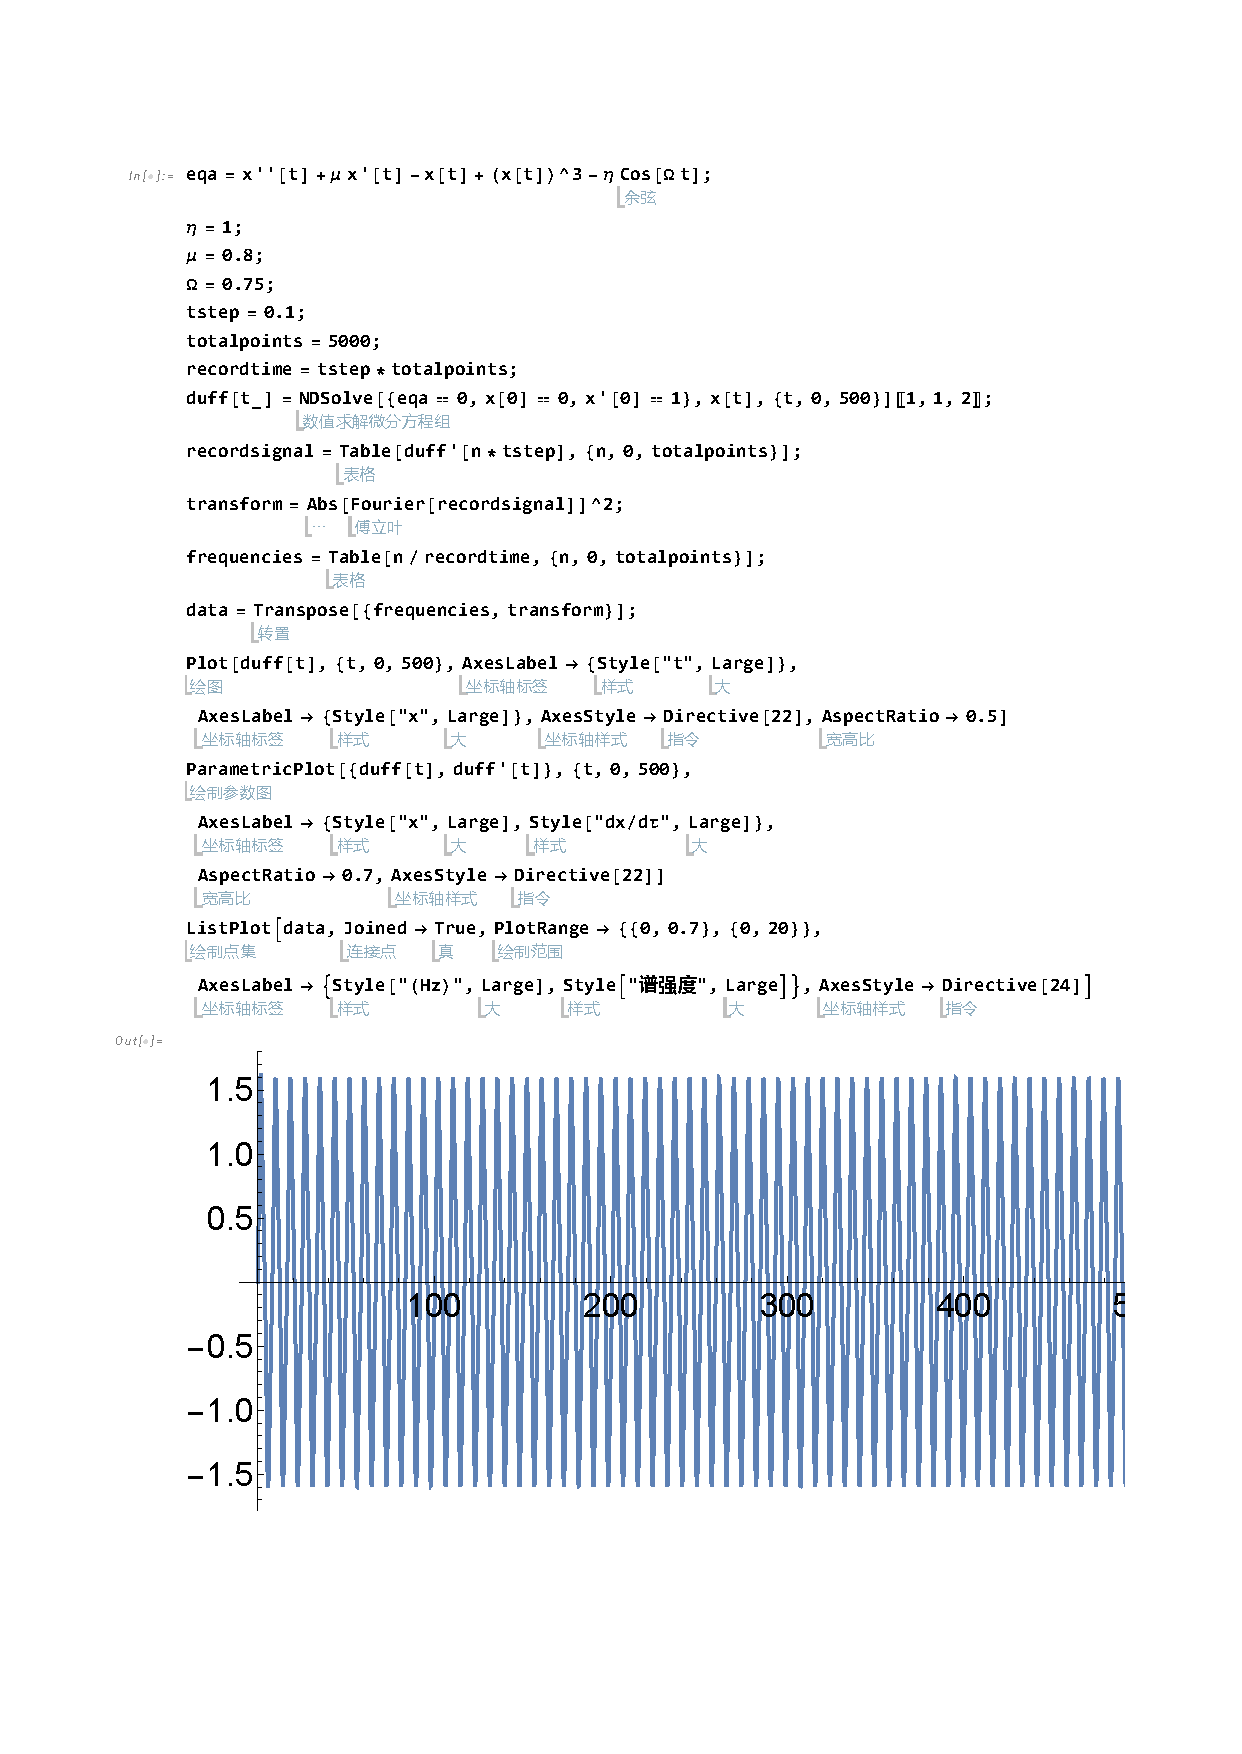
\includepdf[pages=-]{chaos.pdf}
\subsection*{原件扫描}
\includepdf[pages=-]{实验5原件.pdf}

\subsection*{桌面}
\begin{figure}[!h]
	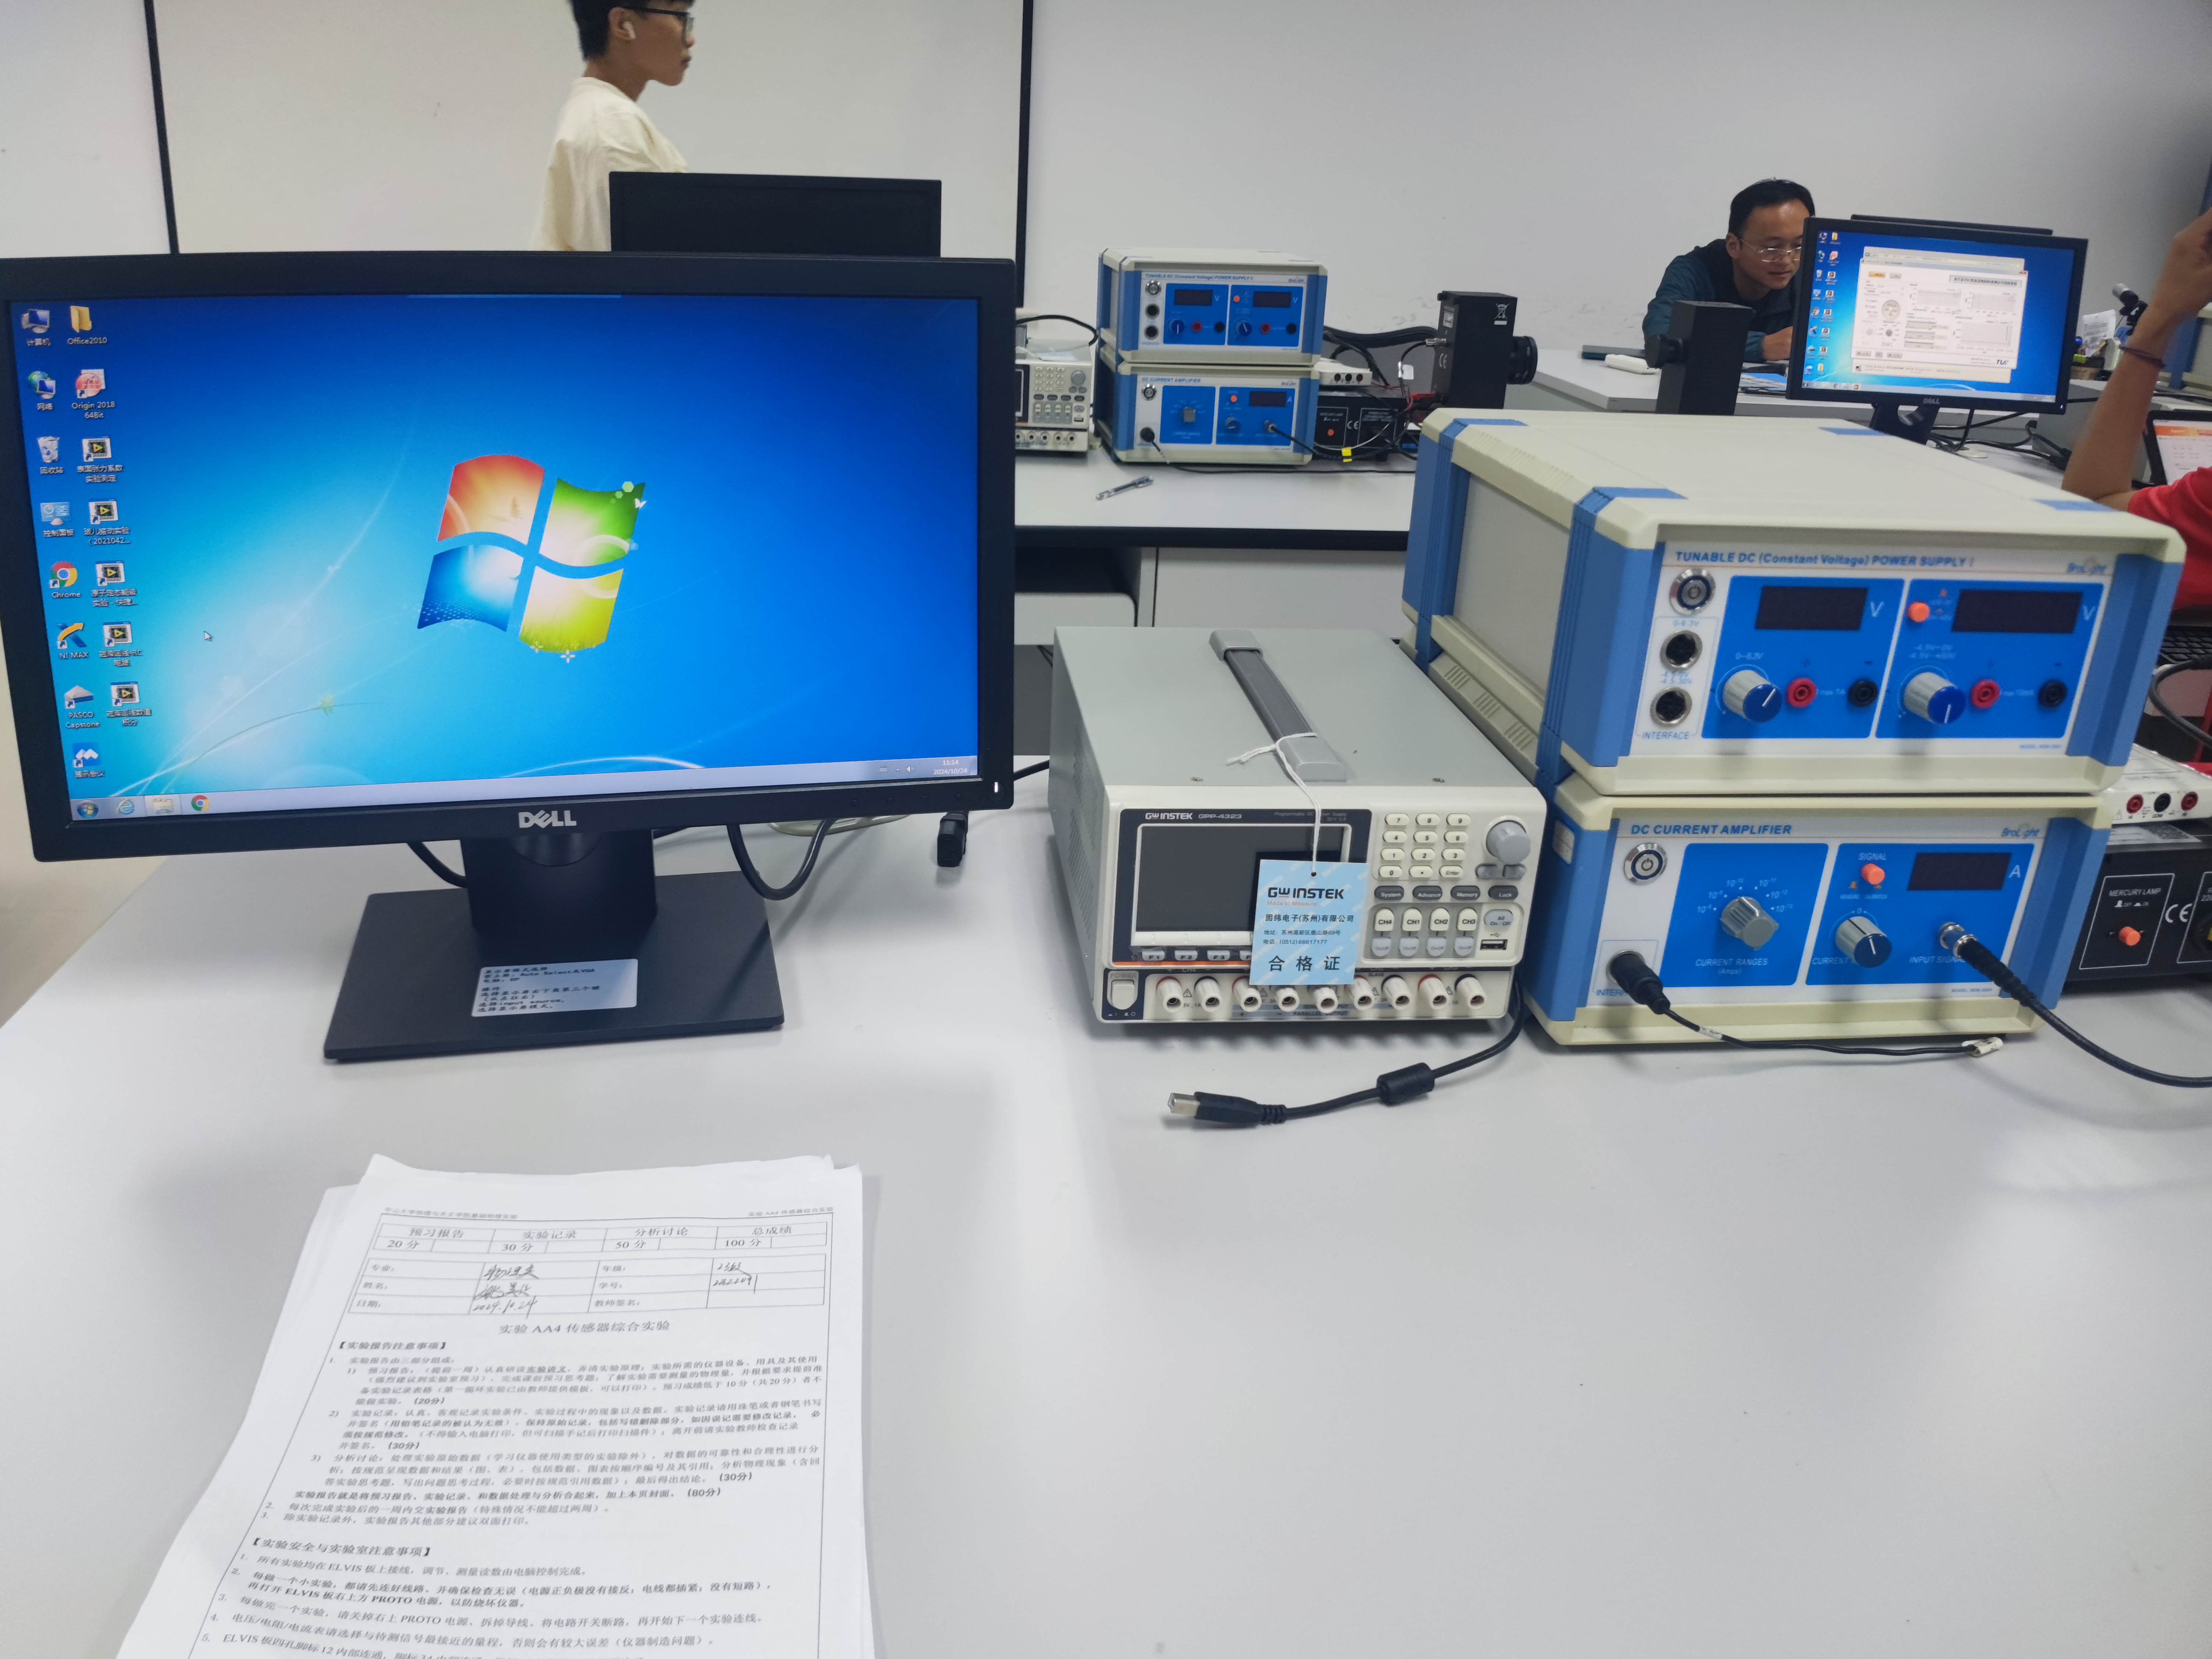
\includegraphics[width=0.95\textwidth]{实验5桌面.jpg}
\end{figure}
\end{document}